\chapter{Design}

\section{System architecture}
\subsection{Interface}
\begin{figure}
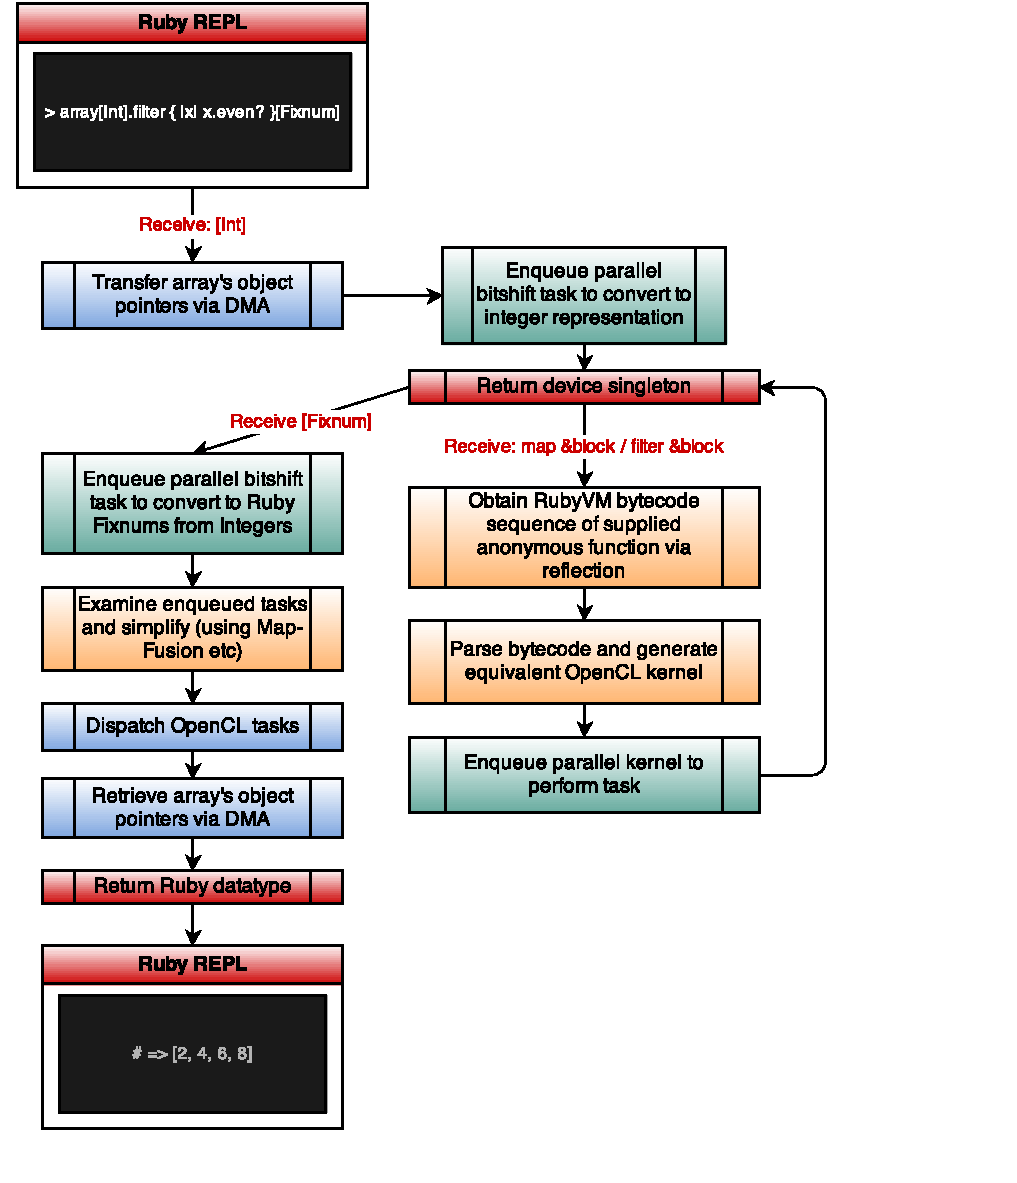
\includegraphics[]{./figures/rubicl_workflow}
  \captionof{figure}{RubiCL execution model.}
    \label{fig:rem}
\end{figure}

The produced system is able to interact seamlessly with existing Ruby code, via type annotation on collection objects.

\begin{lstlisting}[
  language=Ruby,
  label=lst:example_snippet,
  caption=Redirecting a computation through the RubiCL library via type annotation.
]
  # Sequential stdlib code
  (1..1_000_000)
    .map { |x| x + 15 }
    .select { |y| y % 15 == 0 }

  # Parallel code using RubiCL
  (1..1_000_000)[Int]
      .map { |x| x + 15 }
      .select { |y| y % 15 == 0 }[Fixnum]
\end{lstlisting}


When a user is sure that all objects within an \verb|Enumerable| are of a single, basic type, they can append a type declaration to the container. This declaration lies within the method pipeline and states the equivalent C type. The object is then wrapped by the RubiCL execution environment.

Further method calls are swallowed by the \verb|Device| instance handling the dataset, and pushed onto a work-queue.

Eventually, a result is requested. This occurs either by a user casting back to a Ruby object class, or by performing a terminal action such as summation. The work-queue is then optimised and mapped to OpenCL kernels, dispatched to the target compute device.

The produced wrapper solution for including additional functionality to the Ruby runtime is ideal for maintaining usability. Programmers must grasp only the concept of annotating type-conversion at the beginning and end of any calculation pipeline. All other syntax of the library is identical to normally-written Ruby code.

Despite the simplicity of the library's presented interface, there is a lot of work going on behind the scenes. The technical details of which will be discussed over the following $2$ chapters.

As an overview, the steps undertaken by the RubiCL library for the example given in Figure~\ref{lst:example_snippet} include:
\begin{itemize}
  \item Moving the dataset elements into continuous memory, addressable by the compute device.
  \item Recording the loaded dataset type, to allow static type-system operations.
  \item Parsing the \verb|block| argument of the \verb|#map| task's bytecode and constructing an equivalent C99 expression.
  \item Parsing the \verb|block| argument of the \verb|#select| task's bytecode and constructing an equivalent C99 expression.
  \item Inserting a \verb|Map| task at the beginning of the \verb|TaskQueue| to convert from Ruby objects to C \verb|int|s.
  \item Inserting a \verb|Map| task at the end of the \verb|TaskQueue| to convert from C \verb|int|s back to Ruby objects.
  \item Simplifying the $4$ tasks in the \verb|TaskQueue| to a single, \verb|MapFilter| task via \emph{fusion}.
  \item Generating the OpenCL kernel required to perform the \verb|MapFilter| task.
  \item Executing the produced kernel on the compute device, recording metrics.
  \item Releasing resources required by the OpenCL library during the task.
  \item Returning the resultant values as a Ruby array.
\end{itemize}

\subsection{Software architecture}
The library is constructed from the following set of modules and classes, alongside their responsibilities:
\begin{description}
  \item[RubiCL] Environment singleton and top level namespace.
The library's functionality is included in an application by \verb|require|ing this module. It handles the import of all sub-components of the runtime.
Other responsibilities include storing versioning metadata and selecting which available device should be the default compute target.

\paragraph*{Interface:}
\begin{description}
  \item[self.opencl\_device] Returns the current compute device. (The default for this value is \verb|RubiCL::CPU|)
  \item[self.opencl\_device=(Device)] Sets the current compute device.
\end{description}

  \item[CastAccess] A module designed to extend container types, providing the ability to initiate a computation pipeline.
    For example, the Behaviour of the \verb|Array| built-in class is extended by mixing-in the module in the following manner:
\begin{lstlisting}[language=Ruby]
Array.class_eval { include RubiCL::CastAccess }
\end{lstlisting}
This allows parallel primitives performed on \verb|Arrays| to be executed by the compute device following an annotation, such as \verb|[1, 2, 3][Int]|.
Upon casting, the actual conversion operations performed are specified by the target class. This module is decoupled from implementation and provides purely syntactic enhancements.

Traditionally in Ruby, invoking the \verb|[]| method of an \verb|Enumerable| is only used for indexed access to collection members. The standard implementation supports receiving integer arguments and returns the element at the given offset. It also supports \verb|Range| arguments and returns the corresponding continuous subset.

The assumption was made that that providing a \verb|Class| constant as an argument here is something that would never occur in common use. Therefore, the RubiCL library uses occurrences of this calling behaviour to indicate that a dataset should be wrapped.

\paragraph*{Interface:}
\begin{description}
  \item[$\lbrack\rbrack$(Type)] Overridden on extended object to call the conversion method, provided by a \verb|Class| argument's \verb|rubicl_conversion|, on the current compute device, referencing the dataset it was called on. Behaviour when called with a non-\verb|Class| argument is unchanged.
\end{description}

  \item[Target C-type classes]
An observant reader may notice that the constant \verb|Int| is passed in Figure~\ref{lst:example_snippet} when signalling that the container should be transformed into C type \verb|int|s. This class is not defined within the standard library, instead \verb|Fixnum| is the container for fixed-precision integers that can be encoded within a single machine word.

The \verb|Int| class was constructed to represent the abstract type of C integers. In addition, the \verb|Double| type has been defined for double precision floating-point numbers.

Each C-type class defines how to transfer a similarly typed input dataset to the compute device, via methods defined by the \verb|BufferManager|.

\paragraph*{Interface:}
\begin{description}
  \item[self.rubicl\_conversion] Provides the method and type arguments to call on the current compute device, alongside a dataset, in order to load it.
\end{description}

\item[Native Ruby result classes]
At the end of the computation pipeline, results are retrieved either by casting back to a Ruby type, or by performing a terminal action such as summation.

The Ruby classes used to convert back to the calculation's result type are provided with the standard Ruby implementation: \verb|Fixnum| and \verb|Float|.

Mirroring the responsibilities of the C-type classes, additional static methods have been added to these classes to instruct the \verb|BufferManager| how to return a result dataset for the given type.
\paragraph*{Interface:}
\begin{description}
  \item[self.rubicl\_conversion] Provides the method to call on the current compute device, in order to retrieve the typed dataset.
\end{description}

  \item[BufferManager]
In order to prevent the \verb|Device| class becoming a \emph{god object}, manipulating the device buffer is performed through a service object. The \verb|BufferManager| provides an interface to load objects, specifying their C-type, and later retrieve them. The type of the currently loaded buffer is then stored, to assist kernel generation for queued parallel tasks.

The manager also provides caching of the dataset to prevent unnecessary hardware retrieval if no operations have been performed.

The manager's necessary ability to interact with an \ac{OpenCL} buffer is provided by the \verb|BufferBackend| native extension module.
\paragraph*{Interface:}
\begin{description}
  \item[load(type: Type, object: Object)] Makes the provided object addressable by the \ac{OpenCL} compute device.

  \item[retrieve(type: Type)] Retrieves the resultant object from the compute device address space.

  \item[access(type: Type)] Returns a handle to the device address space, passed by \verb|Device| when executing tasks.
\end{description}

\item[Device]
  An abstract superclass, providing all functionality of the execution context during a method pipeline. Instantiated as a singleton, in either \ac{GPU} or \ac{CPU} flavour. The subclass overrides only the initialisation procedure, passing the correct device-type flags to the \ac{OpenCL} \ac{API}, and provides a means to later differentiate between device types. Knowing what type of hardware device a kernel will execute on allows specific optimisations, such as avoiding \emph{bank conflicts} for \verb|Scan| tasks occurring on a \verb|GPU|.
\paragraph*{Interface:}
Where possible, all methods return the device context to allow method chaining.
\begin{description}
  \item[$\lbrack\rbrack$(Type)] Used to signal the end of a computation pipeline. Sends the method provided by \verb|Type.rubicl_conversion| to itself.

  \item[load\_object(Type, Object)] Delegates to the buffer manager.

  \item[retrieve\_integers] Delegates to the buffer manager.

  \item[retrieve\_doubles] Delegates to the buffer manager.

  \item[sort] Enqueues a task to sort the buffer.

  \item[zip(Enumerable)] Flushes the current pipeline, then creates a tuple buffer from the result and the inputted \verb|Enumerable|.

  \item[fsts] Bifurcates a loaded tuple buffer, keeping only the first elements.

  \item[snds] Like the previous method, but keeps only the second elements.

  \item[braid(\&Block)] Collapses a buffer containing a list of tuples into a list of single values, using the provided combination function.

  \item[map(\&Block)] Mutates all elements within the buffer using the provided function.

  \item[filter(\&Block)] Rejects elements from the buffer that do not pass the provided predicate function. Aliased also as \verb|select| to be consistent with the Ruby standard library.

  \item[scan(Style, Pperator)] Produces an array of intermediate results, equivalent to traversing the array and applying the reduction operator up until each point. Inclusive or exclusive option set via parameter, inclusive by default.


  \item[sum] Returns the summation of all values in the buffer.

  \item[count(Value?, \&Block? )] If provided with a value, returns the number of times that the given value appears in the buffer. If provided with an anonymous function, returns the number of values in the buffer that satisfy the predicate. If no arguments are provided, returns the length of the buffer.
\end{description}

\item[LambdaBytecodeParser]
Receives an anonymous Ruby function during instantiation and returns a set of equivalent C expressions on demand. The details of this procedure will be explained in the \emph{Implementation} chapter. This translation stage enables the library to operate when the user states a problem in standard Ruby syntax only.

\paragraph*{Interface:}
\begin{description}
  \item[to\_infix] Returns the function supplied to the constructor in infix form, using C syntax.
\end{description}

\item[Logger]
A singleton used to log key actions to the terminal or disk, facilitating debugging. The current log level set determines whether output will be produced. Enables debug mode to be toggled in a single location.

\paragraph*{Interface:}
\begin{description}
  \item[loud\_mode] Causes any logged actions to be displayed in the terminal.

  \item[quiet\_mode] Ensures logged actions do not appear in the terminal.

  \item[show\_timing\_info=] Toggles whether segmented timing analysis appears before produced computation results.
\end{description}

\item[TaskKernelGenerator]
Instantiated with a \verb|Task| object, the \verb|TaskKernelGenerator| assembles an \ac{OpenCL} kernel performing the task. It handles the majority of \ac{OpenCL} kernel boilerplate, with the task providing only specific computational operations.

\paragraph*{Interface:}
\begin{description}
  \item[create\_kernel] Returns the kernel source for the given task.
\end{description}

\item[Task]
An abstract superclass representing a stage in the computation pipeline. Subclassed with the specific type of operation. Provides tracking of variables required, computation statements and each task's unique name.

\paragraph*{Interface:}
\begin{description}
  \item[descriptor] A pretty-printed description of the task. Provides its name alongside a summary of actions performed.

  \item[to\_kernel] Returns the full \ac{OpenCL} source of the task, obtained through the \verb|TaskKernelGenerator|.

  \item[fuse!(Map)] Present on \verb|Map| tasks, allows a following \verb|Map| task to be combined with the current task.

  \item[fuse!(Filter)] Present on \verb|Filter| tasks, allows a following \verb|Filter| task to be combined with the current task.

  \item[pre\_fuse!(Map)] Present on \verb|MapFilter| tasks, prepends the previous \verb|Map| task's statements to the current task.

  \item[post\_fuse!(Map)] Present on \verb|MapFilter| tasks, appends the following \verb|Map| task's statements to the current task.

  \item[filter\_fuse!(Filter)] Present on \verb|MapFilter| tasks, updates the filtering action to also require the following \verb|Filter| task's predicate to be satisfied.
\end{description}

\item[TaskQueue]
Stores the entire computation pipeline of the current execution chain. Enqueued tasks are appended to the queue. When a result is requested, the entire queue is optimised and then dispatched in as few tasks as possible. The rules for queue optimisation are discussed in the \emph{Implementation} chapter.

\paragraph*{Interface:}
\begin{description}
  \item[push(Task)] Adds a \verb|Task| onto the end of the queue.

\item[shift] Removes the first \verb|Task| from the queue and returns it.

\item[simplify!] Compresses the \verb|TaskQueue| by performing \emph{fusion} optimisations.
\end{description}


\end{description}


\paragraph*{Example interaction} Figure~\ref{fig:rubicl_components} shows the interactions between classes during a typical parallelised computation.
\afterpage{
  \clearpage
  \begin{landscape}
    \begin{figure}[h]
      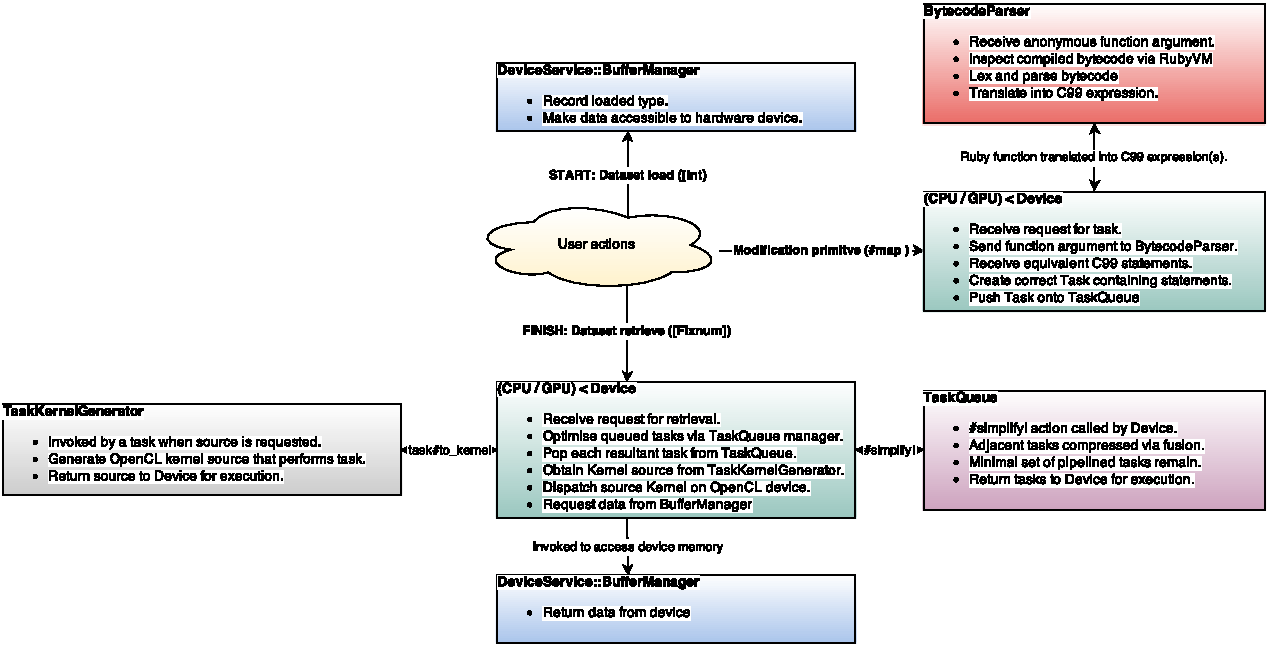
\includegraphics[width=\paperwidth]{./figures/arch_components.pdf}
      \caption{An overview of the interacting software components during the lifetime of a typical computation}
      \label{fig:rubicl_components}
    \end{figure}
  \end{landscape}
}

\subsection{Interacting with hardware devices}
Interaction with hardware devices present on the system occurs via native extensions. These extension modules are mixed-into device singletons, created when the library is first launched. Figure~\ref{fig:rubicl_devices} shows the functionality of these singletons and their subcomponents.

\begin{figure}[h]
  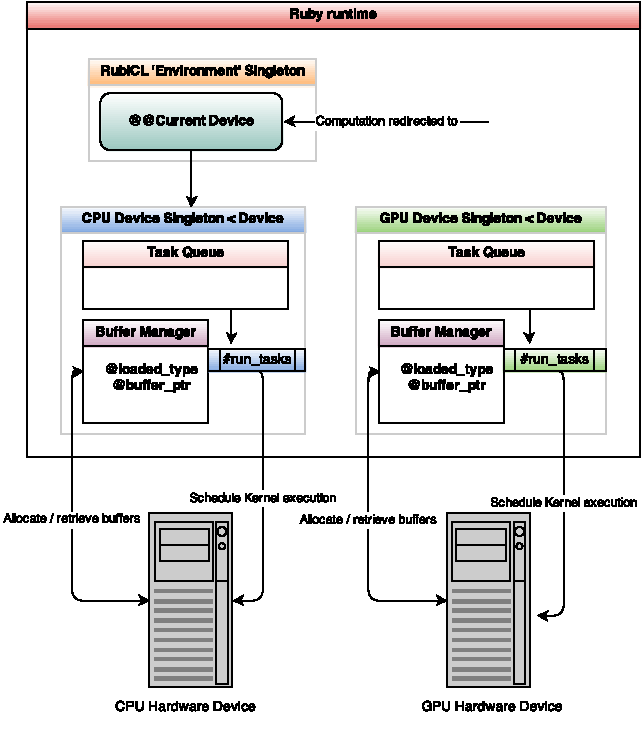
\includegraphics[width=0.8\textwidth]{./figures/arch_diagram.pdf}
  \caption{The RubiCL runtime maintains singletons for each device, used to trigger management functions and execute kernels.}
  \label{fig:rubicl_devices}
\end{figure}

Both \verb|CPU| and \verb|GPU| objects, tasked with managing device state, inherit from a common \verb|Device| superclass. The main difference in their implementation is differing initialisation procedure. Having two device types allows target-specific optimisation by the code generator, shown later.

The \verb|Device| subclasses delegate maintaining the list of tasks to a \verb|TaskQueue| object. In addition, they lack the ability to call memory management functions on devices.
Instead of handling device memory directly, \verb|Device| objects request functionality through an instance of \verb|DeviceService::BufferManager|.

Implementing all device logic that does not require hardware interoperability in Ruby made the system much easier to test. The time taken for the device control flow to execute is insignificant compared to the time taken for data processing. Writing this section in C would have been misguided as the performance benefits would not be worth the impaired rate of development.




\section{Design choices}
\subsection{Type annotation}
When parallelising computation using the RubiCL library, a dataset is initially `cast' to the C-type equivalent. To signify the end of a computation it is finally `cast' back to the Ruby type.

This method of redirecting a method chain using a wrapped object is intentionally similar to \verb|Enumerable#lazy| in Ruby's standard library.

\verb|Enumerable#lazy| allows computation to be deferred until is known how many results are needed. In some cases, such as the example presented in Figure~\ref{lst:example_lazy}, computation can be avoided when the results would be discarded.

\begin{lstlisting}[
  language=Ruby,
  label=lst:example_lazy,
  caption=Redirecting a computation through Enumerable\#lazy.
]
def side_effect_increment(x, str)
  puts str
  x + 1
end

(1..5).map { |x| side_effect_increment x, "Non-lazy" }
    .take_while { |x| x < 4 }
# => [2, 3]

(1..5).lazy
    .map { |x| side_effect_increment x, "Lazy" }
    .take_while { |x| x < 4 }
    .to_a
# => [2, 3]

# Non-lazy invocation evaluates 'side_effect_increment' 5 times:
# >> Non-lazy
# >> Non-lazy
# >> Non-lazy
# >> Non-lazy
# >> Non-lazy
# Lazy invocation evaluates 'side_effect_increment' 3 times:
# >> Lazy
# >> Lazy
# >> Lazy
\end{lstlisting}

Keeping the usage akin to a conceptually similar feature should make the library easier for inexperienced programmers to get to grips with.

\subsection{Eager or deferred task dispatching}
During system design, the decision had to be made whether to eagerly evaluate parallel primitives or to buffer all requests and then dispatch when a result is requested. This choice is not straightforward as there are benefits to either option.

\paragraph*{Advantages of eager dispatch}
\begin{itemize}
\item The kernel build and execution stages can be pipelined. For example, this allows the code generation and compilation stages to execute on the host \ac{CPU} while the previous task is executing on the \ac{GPU}.

\item Compute device can easily be changed mid-chain. Although it will suffer a performance penalty due to the need to transfer the data buffer, having the buffer always in a consistent state allows a device well-suited in a particular primitive to pick up where another left off.

\item Simplicity. No need to study equivalence rules.
\end{itemize}

\paragraph*{Advantages of deferred pipeline}
\begin{itemize}
\item Fewer resultant \verb|Task|s to schedule. Since adjacent combinable tasks are fused, there is less work done by the \ac{OpenCL} compiler and work-group scheduler.

\item Fewer accesses to global device memory. In the setup phase of each kernel, the elements to be transformed are loaded from the global device buffer into local storage. When multiple tasks are combined into one kernel, the intermediate result remains in unsynchronised memory until the task finalizes. This causes much less stress on the compute-device's memory subsystem.

\item Fewer work-units scheduled. It is a waste of iterations to have $3$ \verb|for-loop|s each modify a collection when all operations could occur in a single loop. It is similarly wasteful to execute $N$ work-units $3$ times when only $N$ are needed.
\end{itemize}

The chosen execution style was to defer task requests and then execute optimised tasks when a result is required.

This mirrors the approach taken by many \emph{Object-Relational Mappers}, such as \verb|ActiveRecord|, combining a pipeline of queries into optimal SQL.

The assumption was made that requiring multiple passes over the input dataset was significantly more expensive than the one-off code generation tasks. This was verified by timing information collected during empirical testing:

\subsection{Construction and processing of tuple datasets}
In order to allow a greater variety of query styles to be accelerated, it became clear that tuples should be introduced as a data-type. This necessitated the functionality to load a dataset of tuple elements onto the compute device and support of parallel queries possible on a standard dataset.

After careful consideration of the requirements, two methods of achieving tuple support appeared suitable for the project.

\paragraph*{Custom structures of data for each element} \ac{OpenCL} supports the usage of \verb|struct|s in kernel code. With this in mind, it would be possible to store each tuple continuously in memory and use member access to retrieve each slot. The size of each tuple structure can be used to guide memory management on the host. There are both advantages and disadvantages to this method of implementation. 

An advantage of using structures is the ease of supporting arbitrary length tuples. The host code only knows about the size of each tuple, so that this information can be combined with the number of elements present when allocating the correct amount of device memory. The pre-compiled back-end code has no notion of tuple structure. Only the generated kernel code has the need to interact with slots within a tuple. As such, the structure definition can be generated dynamically at the same point as task definition. 

One disadvantage of using structures is the need to recreate the entire dataset whenever tuples alter length. For example, if an array of 2-element tuples is loaded to the device, and a third slot is added to each, it is necessary to initialize a new buffer and fill it by copying existing values then inserting a new slot value for each tuple. This is the same issue faced when inserting an element within a fixed-size vector. This issue would result in increase cost of the \verb|zip| operator when creating or resizing tuples.

\paragraph*{Virtual tuples stored in disjoint datasets}
When processing tuples of length $2$, instead of creating a buffer storing tuples continuously in memory, two dataset buffers can be provided to each invoked kernel. The first buffer stores the first slot value for each tuple. Likewise, the second buffer stores all second slot values. The generated kernel code can then be designed to operate on tuples as intended, by accessing the indexed value from the buffer corresponding to the slot requested.

This method has the advantage that creation and resizing of tuples is much less expensive. To create tuples, the second dataset, passed as a parameter to the zip operator, is simply provided to subsequent kernel invocations alongside the currently loaded buffer. When resizing tuples, the entire buffer does not need to be recreated because of a shift in individual tuple length. Instead, an extra buffer is passed to all scheduled kernels if the tuple has grown, or one buffer is released and is no longer shared if a slot has been removed.

While this method benefits from greater performance, it is more involved to implement arbitrary sized tuples compared to the previously suggested solution. The host code is now concerned with many disjoint buffers that must be managed and released after use, and all required slots must be provided as kernel arguments prior to scheduling of any execution. In short, the host code is far more coupled to the currently loaded dataset's contents than is desirable.

However, it is clear that the second solution, virtual tuples, achieves greater performance despite a more involved implementation. Therefore, it was chosen as the project's tuple implementation method. The initial implementation of tuples was limited to a $2$ slot maximum so that the design could be completed quickly and verified as correct, but it is entirely possible to expand the system to support arbitrary length tuples later.
